\tikzset{every picture/.style={line width=0.75pt}} %set default line width to 0.75pt

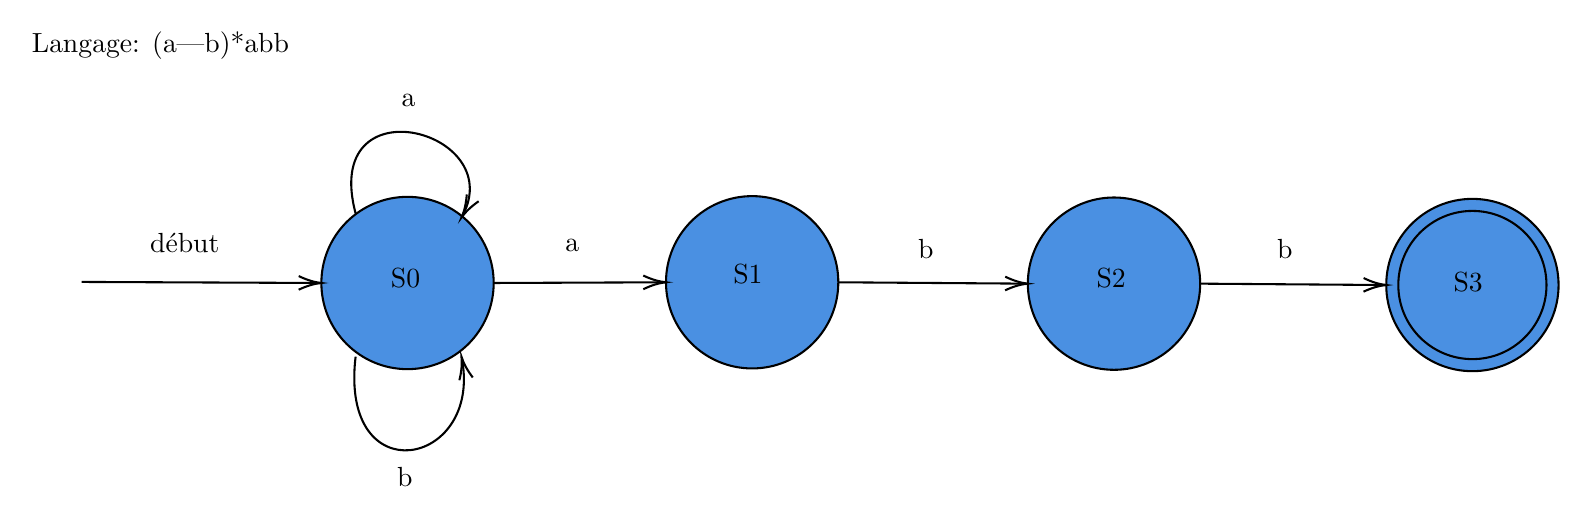
\begin{tikzpicture}[x=0.75pt,y=0.75pt,yscale=-1,xscale=1]
%uncomment if require: \path (0,777); %set diagram left start at 0, and has height of 777

%Shape: Circle [id:dp9851709242772706]
\draw  [fill={rgb, 255:red, 74; green, 144; blue, 226 }  ,fill opacity=1 ] (161,135.51) .. controls (161,112.58) and (179.58,94) .. (202.51,94) .. controls (225.43,94) and (244.02,112.58) .. (244.02,135.51) .. controls (244.02,158.43) and (225.43,177.02) .. (202.51,177.02) .. controls (179.58,177.02) and (161,158.43) .. (161,135.51) -- cycle ;
%Shape: Circle [id:dp2634550867663098]
\draw  [fill={rgb, 255:red, 74; green, 144; blue, 226 }  ,fill opacity=1 ] (327.04,135.17) .. controls (327.04,112.24) and (345.62,93.66) .. (368.55,93.66) .. controls (391.47,93.66) and (410.06,112.24) .. (410.06,135.17) .. controls (410.06,158.09) and (391.47,176.68) .. (368.55,176.68) .. controls (345.62,176.68) and (327.04,158.09) .. (327.04,135.17) -- cycle ;
%Shape: Circle [id:dp7244233597696788]
\draw  [fill={rgb, 255:red, 74; green, 144; blue, 226 }  ,fill opacity=1 ] (501.38,135.83) .. controls (501.38,112.91) and (519.96,94.32) .. (542.89,94.32) .. controls (565.81,94.32) and (584.4,112.91) .. (584.4,135.83) .. controls (584.4,158.76) and (565.81,177.34) .. (542.89,177.34) .. controls (519.96,177.34) and (501.38,158.76) .. (501.38,135.83) -- cycle ;
%Shape: Circle [id:dp07451760427696097]
\draw  [fill={rgb, 255:red, 74; green, 144; blue, 226 }  ,fill opacity=1 ] (674.06,136.49) .. controls (674.06,113.57) and (692.64,94.98) .. (715.57,94.98) .. controls (738.49,94.98) and (757.08,113.57) .. (757.08,136.49) .. controls (757.08,159.42) and (738.49,178) .. (715.57,178) .. controls (692.64,178) and (674.06,159.42) .. (674.06,136.49) -- cycle ;
%Shape: Ellipse [id:dp8941531755272224]
\draw  [fill={rgb, 255:red, 74; green, 144; blue, 226 }  ,fill opacity=1 ] (679.87,136.49) .. controls (679.87,116.78) and (695.85,100.79) .. (715.57,100.79) .. controls (735.28,100.79) and (751.26,116.78) .. (751.26,136.49) .. controls (751.26,156.21) and (735.28,172.19) .. (715.57,172.19) .. controls (695.85,172.19) and (679.87,156.21) .. (679.87,136.49) -- cycle ;
%Straight Lines [id:da9727164886338506]
\draw    (45.5,135) -- (159,135.5) ;
\draw [shift={(161,135.51)}, rotate = 180.25] [color={rgb, 255:red, 0; green, 0; blue, 0 }  ][line width=0.75]    (10.93,-3.29) .. controls (6.95,-1.4) and (3.31,-0.3) .. (0,0) .. controls (3.31,0.3) and (6.95,1.4) .. (10.93,3.29)   ;
%Straight Lines [id:da38657510871619216]
\draw    (244.02,135.51) -- (325.04,135.18) ;
\draw [shift={(327.04,135.17)}, rotate = 539.77] [color={rgb, 255:red, 0; green, 0; blue, 0 }  ][line width=0.75]    (10.93,-3.29) .. controls (6.95,-1.4) and (3.31,-0.3) .. (0,0) .. controls (3.31,0.3) and (6.95,1.4) .. (10.93,3.29)   ;
%Straight Lines [id:da45803946933994955]
\draw    (410.06,135.17) -- (499.38,135.82) ;
\draw [shift={(501.38,135.83)}, rotate = 180.41] [color={rgb, 255:red, 0; green, 0; blue, 0 }  ][line width=0.75]    (10.93,-3.29) .. controls (6.95,-1.4) and (3.31,-0.3) .. (0,0) .. controls (3.31,0.3) and (6.95,1.4) .. (10.93,3.29)   ;
%Straight Lines [id:da19707808507116387]
\draw    (584.4,135.83) -- (672.06,136.48) ;
\draw [shift={(674.06,136.49)}, rotate = 180.42] [color={rgb, 255:red, 0; green, 0; blue, 0 }  ][line width=0.75]    (10.93,-3.29) .. controls (6.95,-1.4) and (3.31,-0.3) .. (0,0) .. controls (3.31,0.3) and (6.95,1.4) .. (10.93,3.29)   ;
%Curve Lines [id:da7298553041692105]
\draw    (177.5,102) .. controls (160.67,38.64) and (250.67,61.53) .. (229.19,102.75) ;
\draw [shift={(228.5,104)}, rotate = 299.74] [color={rgb, 255:red, 0; green, 0; blue, 0 }  ][line width=0.75]    (10.93,-3.29) .. controls (6.95,-1.4) and (3.31,-0.3) .. (0,0) .. controls (3.31,0.3) and (6.95,1.4) .. (10.93,3.29)   ;
%Curve Lines [id:da9993413766624407]
\draw    (177.5,171) .. controls (169.58,237.33) and (238.11,224.27) .. (228.81,172.58) ;
\draw [shift={(228.5,171)}, rotate = 438.27] [color={rgb, 255:red, 0; green, 0; blue, 0 }  ][line width=0.75]    (10.93,-3.29) .. controls (6.95,-1.4) and (3.31,-0.3) .. (0,0) .. controls (3.31,0.3) and (6.95,1.4) .. (10.93,3.29)   ;

% Text Node
\draw (198,43) node [anchor=north west][inner sep=0.75pt]   [align=left] {a};
% Text Node
\draw (277,113) node [anchor=north west][inner sep=0.75pt]   [align=left] {a};
% Text Node
\draw (447,113) node [anchor=north west][inner sep=0.75pt]   [align=left] {b};
% Text Node
\draw (620,113) node [anchor=north west][inner sep=0.75pt]   [align=left] {b};
% Text Node
\draw (196,223) node [anchor=north west][inner sep=0.75pt]   [align=left] {b};
% Text Node
\draw (20,13) node [anchor=north west][inner sep=0.75pt]   [align=left] {Langage: (a|b)*abb};
% Text Node
\draw (77,110) node [anchor=north west][inner sep=0.75pt]   [align=left] {début};
% Text Node
\draw (193,127) node [anchor=north west][inner sep=0.75pt]   [align=left] {S0};
% Text Node
\draw (358,125) node [anchor=north west][inner sep=0.75pt]   [align=left] {S1};
% Text Node
\draw (533,127) node [anchor=north west][inner sep=0.75pt]   [align=left] {S2};
% Text Node
\draw (705,129) node [anchor=north west][inner sep=0.75pt]   [align=left] {S3};

\end{tikzpicture}
